%The title of Chapter 1 shall be Introduction.  It shall justify and highlight the problem 
%posed,  define the topic and explain the aim and scope of the work presented in the thesis.  It 
%may also highlight the significant contributions from the investigation.


With widespread adoption of virtualization\index{Virtualization} 
for hosting applications,
service providers (like Amazon EC2~\cite{ec2}) can facilitate better 
performance isolation, security and elastic resource provisioning.
A virtualization-based provisioning model is attractive for both 
providers\textemdash{}multiplex resources among several customers, and 
clients\textemdash{}\textit{pay-per-use}, use and pay for only as much resource 
as required. Instances of both 
\emph{public}~\cite{ec2}\index{Public cloud} and \emph{private}
Clouds~\cite{ubuntu-private-cloud, ubuntu-cloud-tools} 
exist\index{Private cloud}, which leverage 
virtual machines\index{Virtual machine}
for flexible provisioning.

Several issues, some of which are\textemdash{}mapping of 
resource requirements
from physical to virtual environments~\cite{profiling-and-modeling},
placement policies for virtual machines~\cite{autonomic-vm-placement},
dynamic resource provisioning~\cite{autonomic-virtual-resource-management},
runtime consolidation and migration~\cite{sandpiper},
storage provisioning and access management~\cite{ip-networked-storage}
need to be addressed to provision applications in virtual execution
environments. Further, these problems
need to be addressed in the context of meeting service level
agreements (SLAs)\nomenclature{SLA:}{Service Level Agreement}\index{SLA}
and resource guarantees~\cite{managing-sla-violations},
and simultaneously maximizing the resource multiplexing potential.
\textit{Server consolidation} and 
\textit{dynamic resource provisioning}\index{Provisioning} 
\cite{autonomic-vm-placement}, \cite{autonomic-virtual-resource-management}, 
\cite{sandpiper}, \cite{capacity-management} are
virtual machine migration-enabled\index{Migration} 
techniques aimed to reduce provider-side
resource sprawl and to address elastic 
resource requirements, respectively.

Since application demands are expectedly continuously varying, resource
requirements will also be correspondingly elastic~\cite{ec2}. To support this,
virtualization-based services require automated and dynamic resource
provisioning~\cite{sandpiper}\index{Provisioning}.
Specifically, if a physical machine faces an explosion of resource
requirements, one or more of its 
virtual machines\index{Virtual machine} may need to be
\textit{migrated} to other physical machines for load 
balancing~\cite{entropy, load-balancing} and 
meeting SLA guarantees~\cite{managing-sla-violations}. 
Thus, \textit{dynamic resource provisioning} is possible by 
scaling resources~\cite{smartscale} on the same physical
machine (when physical machine\index{Physical machine}
has sufficient resources to accommodate increased demands)
or by migrating VM\index{VM} to 
another PM\index{PM} with 
sufficient resources (when source PM has 
insufficient resources).

It is widely acknowledged~\cite{capacity-planning, emerging-research-directions}
that the average utilization
levels in a datacenter\index{Datacenter} is around 20\%, that is to say,
the peak-to-average utilization ratios are very high. Typically,
under periods of high load, a VM may be allocated to a single PM of its
own, and when the load falls back down, it may be moved back to another
non-idle PM, such that the total resource utilization needs are
fulfilled on the target PM, and no SLAs\index{SLA} are 
breached of either the VM under
consideration, or the VMs\index{VM} 
that were already executing on the target PM\index{PM}. This
strategy, known as \textit{Server Consolidation}~\cite{grouping-ga, 
two-stage-heuristic, performance-eval, 
LQR-varsha}\index{Server consolidation},
allows under-utilized physical machines\index{Physical machine} 
to be switched off,
thereby saving power and cooling costs. 
This idea is illustrated briefly in Fig.~\ref{consolidation-migration}.

% \begin{figure}[t]
% \begin{center}
% \noindent\makebox[\textwidth]{% 
% \begin{tabular} {cc}
% 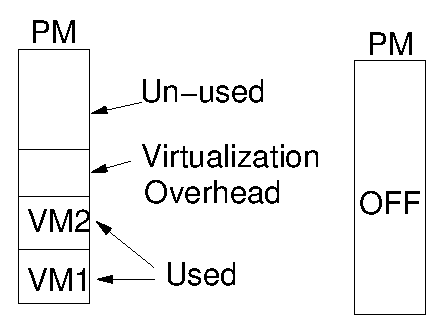
\includegraphics[scale=0.55]{presyn-figures/initially-consolidated.eps} & 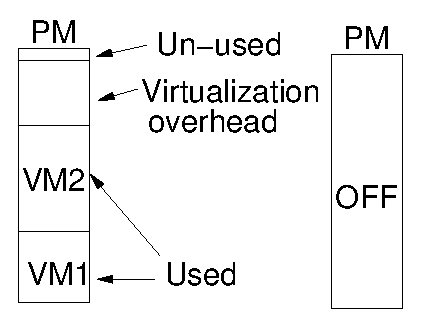
\includegraphics[scale=0.55]{presyn-figures/slight-load-increase.eps} \\
% (a) Initially VMs colocated on a single PM &  (b) Slight increase in load can be accommodated. \\
% 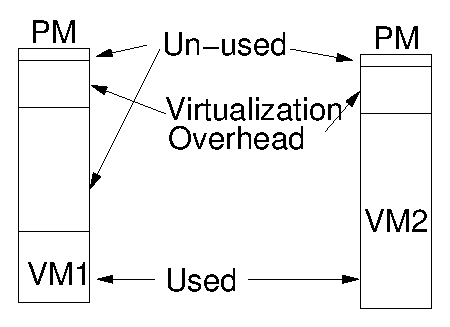
\includegraphics[scale=0.55]{presyn-figures/heavy-load-needs-migration.eps} & 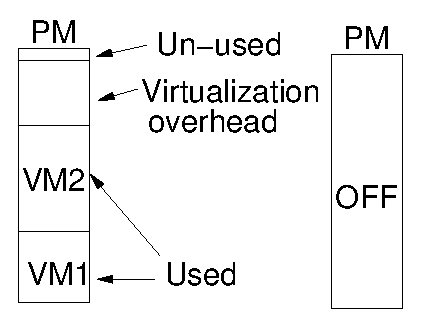
\includegraphics[scale=0.55]{presyn-figures/low-load-migrate-back.eps} \\
% (c) Heavy load requires migration of one VM. & (d) Migrate back when load falls. \\
% \end{tabular}}
% \caption{Server Consolidation and Migration for Dynamic Resource Provisioning.}
% \label{consolidation-migration}
% \end{center}
% \end{figure}

\begin{figure}[t]
\begin{center}
% \noindent\makebox[\textwidth]{% 
\subfloat[VMs colocated on single PM]{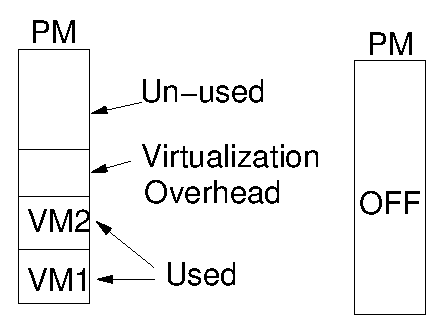
\includegraphics[scale=0.75]{presyn-figures/initially-consolidated.eps}} ~~~~~~~~~~~~~~~~~~~~~~~~
\subfloat[Slight load increase handled]{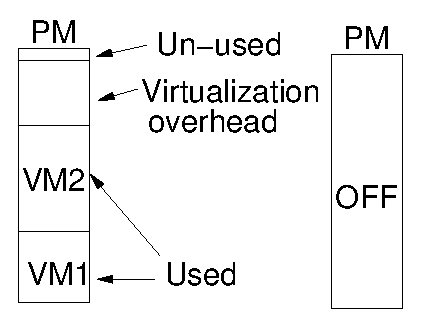
\includegraphics[scale=0.75]{presyn-figures/slight-load-increase.eps}} \\ \vspace{0.15in}
\subfloat[Heavy load requires VM migration]{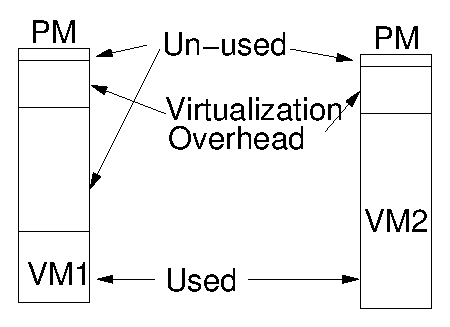
\includegraphics[scale=0.75]{presyn-figures/heavy-load-needs-migration.eps}} ~~~~~~~~~~~~~~~~~~~~~~~~
\subfloat[Migrate back when load falls]{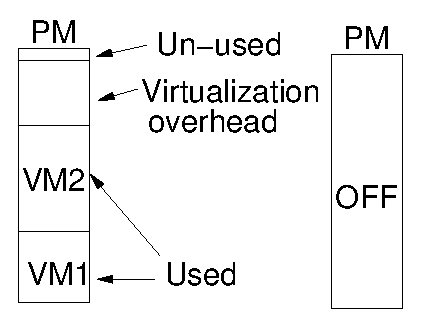
\includegraphics[scale=0.75]{presyn-figures/low-load-migrate-back.eps}}
\vspace{-0.1in}
\caption{Server consolidation and migration for dynamic resource provisioning}
\label{consolidation-migration}
\end{center}
\end{figure}



Most web-based applications are multi-tiered\index{Multi-tiered} and 
virtualization\index{Virtualization}
offers the possibility of hosting each of these tiers (e.g., the 
web-server tier,
the application logic tier and the database server) on separate
elastically provisionable virtual machines. Such differentiated hosting
for various tiers is preferable %to hosting the entire 
%application as a monolithic entity hosted on a single peak-provisioned 
%physical machine since 
as it enables independent resource management and
administration of the different tiers. Additionally, due to
elastic potential of resource allocation to virtual machines,
differentiated hosting on virtual machines can help avoid resource
wastage on under-utilized physical machines.
When applications are instantiated in a virtual
environment, the following major factors affect their 
performance\textemdash{}available network capacity, disk access bandwidth
and virtualization overheads. 


When multiple virtual machines\index{Virtual machine} 
are placed on a single physical machine\index{Physical machine},
they compete for resources like CPU, memory, network and disk I/O
and interact in many conflicting ways. 
% Hence, given a set of physical
% machines, a bin-packing problem would need to be formulated to determine
% which subset of virtual machines need to be placed/co-hosted/consolidated
% on each physical machine, to obtain an optimal placement mapping.
In any virtualized environment, the resources available can 
be broadly categorized into two.

\paragraph{I. Resources allocated to the virtual machines.}
Every virtual machine has access to a set of resources, similar
to those available on physical machines.
For example, virtual CPU, VM page cache, virtual disk, etc.
These are
usually statically allocated in today's datacenters~\cite{ec2},
but can be better managed using dynamic provisioning\index{Provisioning}
techniques~\cite{sandpiper, google-live-migration}.

\paragraph{II. Resources in the virtualized host.} These are resources
at the disposal of the virtualized host to support and enable
the functioning of the hosted VMs. For example, apart from 
the virtual CPU allocated to the VMs, the hypervisor\index{Hypervisor} 
and/or Dom0\index{Dom0} 
also need certain CPU allocation to handle the virtualization
overheads~\cite{measuring-cpu-overhead}. 
Similarly, the virtualized host has a 
page cache\index{Page cache} which is used for managing the buffering of 
physical I/O access~\cite{my-cache-or-yours}. 
\\
\\
In this thesis, we address two
important issues related to the management of both
these types of resources more efficiently, towards the overall goal
of optimizing the performance of virtualized applications.

\section{Thesis contributions}
This thesis addresses problems related to improved resource provisioning
and utilization in virtualized environments. In this section, we concretely
state our contributions.

\paragraph{1. Affinity-aware Modeling of CPU usage for Virtualized Applications.}
The first component of this thesis deals with managing the network 
resource usage of virtual machines and estimating the resulting CPU 
requirement on both the virtual machine\index{Virtual machine} 
and its host system.
Since different tiers of an application require network
communication with each other, placing communicating virtual
machines on the same physical machine\index{Physical machine} 
would reduce physical network 
usage. We define the presence of network traffic between a pair
of VMs as their \textit{network affinity}\index{Network affinity}, 
and state that the
nature of this network traffic is \textit{mutable}\index{Mutable} 
(i.e., changing) based on
whether the VMs are colocated\index{Colocated} or 
dispersed\index{Dispersed}. In other words, the
nature of the network traffic between a pair of VMs
can change between being
intra-PM\index{Intra-PM} and inter-PM\index{Inter-PM} 
depending on whether the VMs are hosted
on the same physical machine or on different physical machines.
We explore the effect of \textit{mutable}
network traffic on CPU usage of colocated and dispersed VMs. More
specifically, the question is, \textit{is the CPU utilization of mutually
communicating VMs dependent on whether the communication happens
intra-PM or inter-PM, and if so, 
how to estimate the target scenario's CPU utilization?}
We make the case that there is significant change in CPU resource
usage of communicating VMs when they are colocated versus when they are 
dispersed, and it is
essential to capture such changes via a model, to assist in
automated server consolidation\index{Server consolidation} 
and VM placement decisions.

We present benchmarking\index{Benchmarking} experiments
which demonstrate impact due to network affinity
on CPU usage of virtual machines and their hosts, when communicating
VMs are colocated as compared to
when they are dispersed. Motivated by these findings, we develop models
that can estimate the ``colocated'' CPU resource usage when VMs transition
from dispersed to colocated placements, and can estimate the ``dispersed''
CPU resource usage when VMs transition from colocated to dispersed
placements. These models predict CPU usage in target 
scenario (colocated/dispersed) based on resource usage profiles 
from source scenario (dispersed/colocated).
First we built models to predict total CPU usage for target scenario,
based on all resource usage profiles like CPU, disk, mutable network
and immutable network usage. However, the maximum error with these 
predictions was found to be around 4 to 6\% absolute CPU usage. 
Hence, based on our findings that CPU usage is affected only by
\textit{mutable} network traffic levels, we build models to 
predict the difference in (or differential) CPU usage based on only
the mutable network traffic profiles. These models were much more
accurate, with maximum error within 2\%. Finally, we applied these
pair-wise models to multi-VM scenarios using a multi-phase
prediction methodology. This demonstrated that simple models
built on the scale of two VMs could be successfully used to
predict for multi-VM scenarios as well.

\paragraph{2. Using Implicit Caching Hints for {D}isk I/O {R}eduction in Virtualized Environments.}\index{DRIVE}
This component deals with managing the cache resource
usage on a virtualized host machine so as to improve the disk access performance 
of the virtual machines.
Due to increased permeation of virtualization-based systems, there is a lot of 
inherent content similarity in systems like email servers, web servers 
and file servers. All this data resides on disk and is fetched by corresponding
applications, as and when required. 
Typically, caches are addressed by block number (hence called 
\textit{block-based} caches)\index{Block-cache} and are not
equipped to recognize content similarity across multiple blocks.
Harnessing the content similarity can help 
avoid duplicate disk I/O requests that fetch the same content repeatedly.
In this work, we incorporate intelligent I/O redirection within the 
storage virtualization engine of the device to manage the underlying 
block-based cache like a \textit{content-deduplicated} cache.

We build a disk read-access optimization called DRIVE, that
identifies content similarity across multiple blocks, and performs
hint-based read I/O redirection to improve cache effectiveness,
thus reducing the number of disk reads further.
% than other systems.
A metadata store is maintained based on the virtual machine's disk
accesses and implicit caching hints are collected
for future read I/O redirection\index{I/O redirection}.
The read I/O redirection is performed from within the virtual
block device in the virtualized system, to manipulate the entire
host-cache as a content-deduplicated cache implicitly.
Our trace-based evaluation using a custom simulator\index{Simulator}, 
reveals that
DRIVE always performs equal to or better than the Vanilla system,
achieving up to 20\% better cache-hit ratios and reducing the
number of disk reads by up to 80\%. The results also indicate that
our system is able to achieve up to 97\% content 
deduplication\index{Deduplication} in the host-cache.

\section{Tools and deliverables}
As part of the work in this thesis, we developed several tools and utilities,
that we report here as ``deliverables'' of this thesis. For each of these
tools, their motivation, requirements specification, design and 
implementation are discussed in the Appendix chapters.
\begin{enumerate}
	\item \texttt{LoadGen}: This is a multi-threaded workload generator, 
		that can be used to generate various types of worklaods like
		CPU, disk, network and mixed workloads at pre-specified levels.
		For details, refer to Appendix Chapter~\ref{chap:thesis-loadgen}.
	\item \texttt{SimReplay}: This is a custom cache simulator, with 
		extensions to look into content similarity while operating 
		the cache. For details, refer to Appendix 
		Chapter~\ref{chap:thesis-simreplay}.
	\item \texttt{Preadwritedump}: This is an I/O trace logging and
		collection toolkit, consisting of different tools to perform
		I/O tracing in the Linux kernel and for collecting the logs
		from the kernel datastructures and writing 
		into the persistent filesystem. For details, refer to Appendix 
        Chapter~\ref{chap:thesis-tracing}.
\end{enumerate}

\section{Thesis outline}
The rest of this thesis is organized as follows. 
Chapter~\ref{chap:thesis-litreview} presents brief background 
to cover the scope of this thesis.
In Chapter~\ref{chap:thesis-arescue}, we present work
related to building affinity-aware CPU estimation\index{Estimation} models 
for migrating VMs and their hosts. In Chapter~\ref{chap:thesis-drive},
we present our I/O reduction system called DRIVE\index{DRIVE} which
improves the efficiency of host cache using deduplication-based
I/O redirection. For further evaluation of DRIVE, we 
performed a detailed literature survey comprising over 100+
publications and 350+ datasets. So, in 
Chapter~\ref{chap:thesis-architecting},
we present the findings of our survey, 
which shows that there are no realistic I/O workload datasets 
or benchmarks available that captures content representation.
In Chapter~\ref{chap:thesis-open-directions}, we present
some open directions and future work for this thesis,
and Chapter~\ref{chap:thesis-conclusions} concludes.

